\subsection{Motivation (Vectors in 3-space)}

\begin{tcolorbox}[title=Problem 1, breakable]
    Given the point $P = (2, -1, 3)$ and the vector 
        $u = [-3, 4, 5]$, find the point $Q$
        such that $\overrightarrow{PQ} = u$.
\end{tcolorbox}

\begin{proof}
    We require $\vec{u} = [-3, 4, 5] = (q_1 - 2, q_2 - (-1), q_3 - 3)$.
    Solving componentwise, we see $(q_1, q_2, q_3) = (-1, 3, 8)$.
    Thus, $Q = (-1, 3, 8)$.
\end{proof}


\begin{tcolorbox}[title=Problem 2, breakable]
    Given the points $P(2, -1, 3)$, $Q(3, 4, 1)$,
        $R(4, -3, 4)$, $S(5, 2, 2)$. True or false (explain:)
        $PQSR$ is a parallelogram.
\end{tcolorbox}

\begin{proof}
For $PQSR$ to be a parallelogram, we require $\vec{PQ} = \vec{SR}$.
$$
\vec{PQ} = [3 - 2,\; 4 - (-1),\; 1 - 3] = [1, 5, -2]
$$
$$
\vec{SR} = [4 - 5,\; -3 - 2,\; 4 - 2] = [-1, -5, 2]
$$
Since
$$
[1, 5, -2] \neq [-1, -5, 2],
$$
it follows that $PQSR$ is not a parallelogram.
\end{proof}

\begin{tcolorbox}[title=Problem 4, breakable]
    Show that for every triple points $P, Q, R$,
        $\overrightarrow{PQ} + \overrightarrow{QR} = \overrightarrow{PR}$.
    [Method $1$: Calculate components. Method 2: Draw a picture.]
\end{tcolorbox}

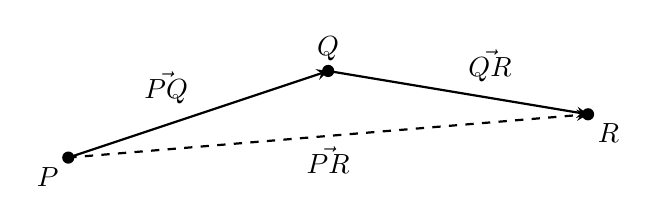
\begin{tikzpicture}[scale=1.1, >=stealth]
    % Points
    \coordinate (P) at (0,0);
    \coordinate (Q) at (3,1);
    \coordinate (R) at (6,0.5);

    % Dots
    \fill (P) circle (2pt) node[below left] {$P$};
    \fill (Q) circle (2pt) node[above] {$Q$};
    \fill (R) circle (2pt) node[below right] {$R$};

    % Vectors
    \draw[->, thick] (P) -- (Q) node[midway, above left] {$\vec{PQ}$};
    \draw[->, thick] (Q) -- (R) node[midway, above right] {$\vec{QR}$};
    \draw[->, thick, dashed] (P) -- (R) node[midway, below] {$\vec{PR}$};
\end{tikzpicture}

\subsection{$\mathbb{R}^n$ and $\mathbb{C}^n$}

\begin{tcolorbox}[title=Problem 2, breakable]
    Consider the vectors 
        $u = (2, 1)$, $v = (-5, 3)$, $w = (3, 4)$
            in $\mathbb{R}^2$.
    Do there exists real numbers $a, b$
        such that $au + bv = w$?
    What if $v = (6, 3)$.
\end{tcolorbox}

\begin{proof}
    We require $au + bv = w
    \iff a(2, 1) + b(-5, 3) = (3, 4)
    \iff (2a, a) + (-5b, 3b) = (3, 4)
    \iff (2a - 5b, a + 3b) = (3, 4)$.
    Thus
    $$
    \begin{cases}
    2a - 5b = 3 \\
    a + 3b = 4
    \end{cases}
    $$
    which has the solution $a = \frac{29}{11},\ b = \frac{5}{11}$.
    If $v = (6, 3)$, we require
    $$
    a(2, 1) + b(6, 3) = (3, 4)
        \iff (2a + 6b, a + 3b) = (3, 4).
    $$
    Thus
    $$
    \begin{cases}
    2a + 6b = 3 \\
    a + 3b = 4
    \end{cases}
    $$
    which has no solution.
    To see this has no solution, note
    $$
    a + 3b = 4 \implies 6b = 8 - 2a.
    $$
    Plugging into the first equation gives
    $$
    2a + (8 - 2a) = 3 \implies 8 = 3,
    $$
    which is a contradiction.
\end{proof}

\begin{tcolorbox}[title=Problem 3, breakable]
    Give a detailed proof of (8) of Theorem 1.2.3 (just checking!).
    [Write out all steps of the proof and give a reason for each step.]
\end{tcolorbox}

\begin{proof}
    Let $x = [x_1, x_2, \ldots, x_n] \in F^n$ be a vector and let $c, d \in F$ where $F$ is a field.  
    Then
    $$
    (cd)x = [(cd)x_1, (cd)x_2, \ldots, (cd)x_n].
    $$
    Since $F$ is a field, scalar multiplication in $F$ is associative thus
    $$
    (cd)x_i = c(d x_i) \quad \text{for each } i = 1, 2, \ldots, n.
    $$
    Therefore,
    $$
    (cd)x = [c(d x_1), c(d x_2), \ldots, c(d x_n)] = c(d x),
    $$
\end{proof}

\begin{tcolorbox}[title=Problem 4, breakable]
    In Definition 1.2.1, $n = 1$ is not ruled out.
    What do the elements of $\mathbb{R}^1$ look like?
    Describe sums and scalar multiples in $\mathbb{R}^1$.
\end{tcolorbox}

\begin{proof}
    The elements of $\mathbb{R}^1$ look like $[x_1]$ where $x_1 \in \mathbb{R}$.  
    Sums and scalar multiples behave identically to the operations in the field $\mathbb{R}$.
\end{proof}

\subsection{Vectors Spaces: The Axioms some Examples}

\begin{tcolorbox}[title=Problem 1, breakable]
    Let $V$ be a vector space over a field $F$.
    Let $T$ be a nonempty set and let $W = \mathcal{F}(T, V)$
    be the set of all functions $x : T \longrightarrow V$.
    Show that $W$ can be made into a vector space over $F$
    in a natural way. [Hint: Use the definitions in Example 1.3.4
    as a guide.]
\end{tcolorbox}

\begin{proof}
    For $x, y \in W$, $x = y$ means that $x(t) = y(t)$ for all $t \in T$.
    If $x, y \in W$ and $c \in F$, define functions $x + y$ and $cx$ by the 
    formulas $(x + y)(t) = x(t) + y(t)$ and $(cx)(t) = c x(t)$ for all $t \in T$.
    Let $\theta$ be the function defined by $\theta(t) = 0$ for all $t \in T$,
    and for $x \in W$, let $-x$ be the function defined by $(-x)(t) = -x(t)$ for 
    all $t \in T$.
\end{proof}

\begin{tcolorbox}[title=Problem 2, breakable]
    The definition of a vector space (1.3.1) can be formulated 
    as follows. A vector space over $F$ is a nonempty set $V$
    together with a pair of mappings $\sigma : V \longrightarrow V$
    and $\mu : F \times V \longrightarrow V$. ($\sigma$ suggests `sum'
    and $\mu$ suggests `multiple') having the following properties 
    $\sigma(x, y) = \sigma(y, x)$ for all $x, y \in V$;
    $\sigma(\sigma(x,y), z) = \sigma(x, \sigma(y, z))$
    for all $x, y, z \in V$ etc. The exercise: Write out the `etc.' in detail.
\end{tcolorbox}

\begin{proof}
    We list the $9$ axioms below:
    \begin{enumerate}
        \item $x,y \in V \implies \sigma(x, y) \in V$
        \item $x \in V, c \in F \implies \mu(c, x) \in V$
        \item $x, y \in V \implies \sigma(x, y) = \sigma(y, x)$
        \item $x, y, z \in V \implies \sigma(x, \sigma(y, z)) = \sigma(\sigma(x, y), z)$
        \item $\exists 0 \in V$ such that $\sigma(0, v) = v = \sigma(v, 0)$
        \item $x \in V \implies -x \in V$ such that $\sigma(x, -x) = 0 = \sigma(-x, x)$
        \item $x, y \in V$ and $c \in F \implies \mu(c, \sigma(x, y)) = \sigma(\mu(c, x), \mu(c, y))$
        \item $\exists 1 \in F$ such that $x \in V \implies \mu(1, x) = x$
        \item $a, b \in F$ and $x \in V \implies \mu(a, \mu(b, x)) = \mu(a b, x)$
    \end{enumerate}
\end{proof}

\begin{tcolorbox}[title=Problem 3, breakable]
    Let $V$ be a complex vector space (1.3.2).
    Show that $V$ is also a real vector space 
    (sums as usual, scalar multiplication restricted to real scalars).
    These two ways of looking at $V$ may be indicated by writing $V_c$ and $V_r$.
\end{tcolorbox}

\begin{proof}
    Clearly $V_r$ is closed under scalar multiplication and vector addiction
        and is a vector space.
\end{proof}

\begin{tcolorbox}[title=Problem 4, breakable]
    Every real vector space $V$ can be `embedded'
    in a complex vector space $W$ in the following way:
        let $W = V \times V$ be the real vector space 
        constructed as in example 1.3.10 and define multiplication 
        by complex scalars by the formula 
        $(a + bi)(x, y) = (ax - by, bx + ay)$
        for $a, b \in \mathbb{R}$ and $(x, y) \in W$.
    [In particular, $i(x, y) = (-y, x)$. Think of $(x, y)$ as `$x + iy$']
    Show that $W$ satisfies the axioms for a complete vector space ($W$ is 
    called the \emph{complexification} of $V$.)
\end{tcolorbox}